\section{Généralisation}
\subsection{Cas avec n communautés}
On peut a présent généraliser à un nombre de communautés $q \geq 2$.
Nous allons supposer que les communautés sont de même taille, à savoir $n_q = \frac{n}{q}$.
\paragraph{}\label{rq:contrainte model}
Une première contrainte apparaît, de par l'utilisation des théorèmes \ref{th:1} et \ref{th:2}, sur les valeurs des probabilités de la matrice d'adjacence $A$.
En effet, d'après le \autoref{th:1}, pour que la matrice $X$ est une mesure spectrale qui tende vers la loi de Wigner il faut que la norme 1 des vecteurs lignes de son profile de variance soient égales ($\parallel x \parallel_1 = \sum_{j=1}^{n}|x_j|$).
Par conséquent, si on veut augmenter le nombre de communautés $q$ dans le modèle, on est forcé de garder deux probabilités $p_{in}$ et $p_{out}$ qui jouent le même rôle que celles introduites précédemment (cf. \ref{rq:probability}).\\

On sait que la matrice d’adjacence du graphe sous le SBM à $q$ communautés est $A = X + \langle A \rangle$.  
Pour poursuivre l'analyse on va suivre la trame suivante:
\begin{itemize}
	\item[1-] Trouver l'équation de $\langle A \rangle$ ;
	\item[2-] Trouvez l'équation de X et déterminer son profile de variance ;
	\item[3-] Trouvez les $q$ valeurs propres associées aux perturbations de rang 1 ;
	\item[4-] Trouver $p_{lim}$.\\
\end{itemize}

% ------------------------------------------------- 1- trouver <A>  -------------------------------------------------
D'une manière générale on trouve que:
\begin{align} 
\langle A \rangle :&= n_q(p_{in} + (q-1)p_{out}) \mathbf{11}^T + n_q\frac{\sqrt{2(q-1)}}{\sqrt{q}}(p_{in}-p_{out})\sum_{i=1}^{q-1}\mathbf{u}_i\mathbf{u'}_i^T\\
				   &= \frac{c_{in} + (q-1)c_{out}}{q} \mathbf{11}^T + \frac{\sqrt{2(q-1)}}{q\sqrt{q}}(c_{in}-c_{out})\sum_{i=1}^{q-1}\mathbf{u}_i\mathbf{u'}_i^T
\end{align}
avec
\begin{align*}
\begin{bmatrix}
\mathbf{1} & \mathbf{u}_1 & \cdots & \mathbf{u}_{q - 1}
\end{bmatrix} 
&=
\begin{bmatrix}
\frac{\mathbf{v}_1}{\parallel \mathbf{v}_1 \parallel} & \frac{\mathbf{v}_2}{\parallel \mathbf{v}_2 \parallel} & \cdots & \frac{\mathbf{v}_q}{\parallel \mathbf{v}_q \parallel}
\end{bmatrix}\\
\begin{bmatrix}
\mathbf{1} & \mathbf{u'}_1 & \cdots & \mathbf{u'}_{q - 1}
\end{bmatrix} 
&=
\begin{bmatrix}
\frac{\mathbf{v'}_1}{\parallel \mathbf{v'}_1 \parallel} & \frac{\mathbf{v'}_2}{\parallel \mathbf{v'}_2 \parallel} & \cdots & \frac{\mathbf{v'}_q}{\parallel \mathbf{v'}_q \parallel}
\end{bmatrix}
\end{align*}
où 
\begin{align*}
\begin{bmatrix}
\mathbf{v}_1 & \mathbf{v}_2 &  \cdots & \mathbf{v}_{q}
\end{bmatrix} 
&=
\begin{bmatrix}
1 & -1 & -1 & \cdots & -1 \\
1 & 1 & 0 & \cdots & 0 \\
\vdots & 0 & \ddots &  & \vdots \\
\vdots & \vdots &  & \ddots & 0 \\
1 & 0 & \cdots& \cdots & 1 \\
\end{bmatrix} \otimes \mathbf{1}_{n_q} \in \mathit{M}_q \otimes \mathit{M}_{n_q\times1}=\mathit{M}_{n\times q}\\
\begin{bmatrix}
\mathbf{v'}_1 & \mathbf{v'}_2 &  \cdots & \mathbf{v'}_{q}
\end{bmatrix} 
&= \frac{1}{n}
\begin{bmatrix}
1 & -1 & -1 & \cdots & -1 \\
1 & q -1 & -1 & \cdots & -1 \\
\vdots & -1 & \ddots &  & \vdots \\
\vdots & \vdots &  & \ddots & -1 \\
1 & -1 & \cdots& \cdots & q-1 \\
\end{bmatrix}\otimes \mathbf{1}_{n_q} \in \mathit{M}_q \otimes \mathit{M}_{n_q\times1}=\mathit{M}_{n\times q}\\
\end{align*}
\begin{align}\label{eq:norm generalize}
\parallel \mathbf{v}_1 \parallel^2 &= \frac{1}{n} & \; & \langle \mathbf{1}  \:|\: \mathbf{u}_i  \rangle = 0 \;,\forall i\nonumber\\
\parallel \mathbf{v}_i \parallel^2 &= \frac{2n}{q} & \; & \langle \mathbf{1} \:|\: \mathbf{u'}_i  \rangle = 0 \;,\forall i \\
\parallel \mathbf{v'}_i \parallel^2 &= \frac{q - 1}{n} & \; & \langle \mathbf{u}_i\:|\: \mathbf{u'}_i  \rangle = \sqrt{\frac{q}{2(q-1)}} \;,\forall i\nonumber\\
 \langle \mathbf{u}_i \:|\: \mathbf{u}_j  \rangle &= \frac{1}{2n} \;,\forall i \neq j & \; & \langle \mathbf{u'}_i \:|\: \mathbf{u'}_j  \rangle = \frac{1}{q - 1} \;,\forall i \neq j \nonumber\\
\langle \mathbf{u}_i \:|\: \mathbf{u'}_j  \rangle &= 0 \;,\forall i \neq j \nonumber
\end{align}\\

% ------------------------------------------------- 2- trouver X  -------------------------------------------------
De la même manière que dans \autoref{ch:Analyse spectrale de la matrice d'adjacence} on trouve:
\begin{equation}
	X_{ij} \sim \left\{
	\begin{array}{lr}
		\sigma_{in} Z_{ij} & : (i,j \in P_{in}) \\
		\sigma_{out} Z_{ij} & : (i,j \in P_{out})
	\end{array}
\right.\nonumber
\end{equation}
Où $Z_{ij} = \frac{B(p) - p}{\sqrt{p(1-p)}} \;\;avec \; p = p_{in} \lor p_{out}$\\
Soit le profile de variance de $\frac{X}{\sqrt{n}}$ et $\sigma^2$ la somme de n'importe quel de ces vecteurs lignes on obtient: 
\begin{align}
\label{eq:sigma2} 
\sigma^2 = \frac{\sigma_{in}^2 + (q-1)\sigma_{out}^2}{q}
\end{align}\\

% ------------------------------------------------- 3- trouver les vp -------------------------------------------------
On va à présent essayer de trouver les $q$ valeurs propres de $A$ associées au perturbations de rang 1. 
Repartons de $A = X + \langle A \rangle$.
\begin{align}
&\Leftrightarrow \frac{A}{\sqrt{n}}v =\lambda v \nonumber \\
&\Leftrightarrow (\Gamma - \lambda I)v =-\alpha \mathbf{11}^Tv - \beta \sum_{i=1}^{q-1}\mathbf{u}_i\mathbf{u'}_i^T \label{eq:generalize}
\end{align}
Pour trouver la valeur propre associée à $\mathbf{11}^T$ on multiplie par à gauche par $\mathbf{1}^T(\Gamma -\lambda I)^{-1}$ et on obtient:
\begin{align}
\eqref{eq:generalize} &\Leftrightarrow \mathbf{1}^Tv =-\alpha \mathbf{1}^T(\Gamma -\lambda I)^{-1}\mathbf{11}^Tv - \beta \mathbf{1}^T(\Gamma -\lambda I)^{-1}\sum_{i=1}^{q-1}\mathbf{u}_i\mathbf{u'}_i^Tv \nonumber\\
&\xrightarrow[n \to +\infty]{} 1 = -\alpha g_{wig}^{\sigma^2}(\lambda) \nonumber\\
&\Leftrightarrow 1 = \alpha \frac{\lambda + \sqrt{\lambda^2 - 4\sigma^2}}{2\sigma^2} \nonumber\\
&\Leftrightarrow \lambda = \frac{c_{in} + (q-1)c_{out}}{q\sqrt{n}} + \frac{q\sqrt{n}\sigma^2}{c_{in} + (q-1)c_{out}} \label{eq:z2 generalize}
\end{align}
Si on remplace $q$ par $2$ on retrouve l'équation \eqref{z2}.\\
Pour trouver les valeurs propres associées aux $\mathbf{u}_i\mathbf{u'}_i^T$ on multiplie par à gauche par $\mathbf{u'}_i^T(\Gamma -\lambda I)^{-1}$ et on obtient:
\begin{align}
\eqref{eq:generalize} &\Leftrightarrow \mathbf{u'}_i^Tv =-\alpha \mathbf{u'}_i(\Gamma -\lambda I)^{-1}\mathbf{11}^Tv - \beta \mathbf{u'}_i(\Gamma -\lambda I)^{-1}\sum_{i=1}^{q-1}\mathbf{u}_i\mathbf{u'}_i^Tv \nonumber\\
&\xrightarrow[n \to +\infty]{} \mathbf{u'}_i^Tv = -\beta(\langle \mathbf{u'}_i\:|\: \mathbf{u}_i \rangle\mathbf{u'}_i^Tv + \sum_{j \neq i}^{} \langle \mathbf{u'}_i\:|\: \mathbf{u}_j \rangle\mathbf{u'}_j^Tv)g_{wig}^{\sigma^2}(\lambda) \nonumber\\
\eqref{eq:norm generalize} &\Rightarrow 1 = -\beta  \sqrt{\frac{q}{2(q-1)}} g_{wig}^{\sigma^2}(\lambda) \nonumber\\
&\Leftrightarrow 1 = \beta \sqrt{\frac{q}{2(q-1)}} \frac{\lambda + \sqrt{\lambda^2 - 4\sigma^2}}{2\sigma^2} \nonumber\\
&\Leftrightarrow \lambda = \frac{c_{in} - c_{out}}{q\sqrt{n}} + \frac{q\sqrt{n}\sigma^2}{c_{in} - c_{out}}\label{eq:z1 generalize}
\end{align}
Si on remplace $q$ par $2$ on retrouve l'équation \eqref{z1}.\\
Nous noterons $z1 =$ \eqref{eq:z1 generalize}  et $z2 =$ \eqref{eq:z2 generalize} pour la suite.
Ces deux équations suffisent à retrouver les probabilités $p_{in}$ et $p_{out}$ du modèle à partir des valeurs propres empiriques (i.e calculées numériquement sur la matrice adjacente du graphe étudié.)\\

% ------------------------------------------------- 4- trouver p_lim -------------------------------------------------
Nous cherchons maintenant à déterminer $p_{lim}$.
La condition limite naturelle est celle où la valeur propre maximale est égale au bord droit du support de la mesure spectrale de la matrice A.
On a alors 
\begin{align*}
	&\Leftrightarrow \lambda^+ = z1\\
	&\Leftrightarrow 2 \sigma = \frac{c_{in} - c_{out}}{q\sqrt{n}} + \frac{q\sqrt{n}\sigma^2}{c_{in} - c_{out}}\\
	&\Leftrightarrow 0 = \beta \sigma^2 - 2 \sigma + \alpha \\
	&\text{après résolution de l'équation on obtient une unique solution}\\
	&\Leftrightarrow p_{in} - p_{out} = \frac{q\sigma}{\sqrt{n}}  \\
\end{align*}
Donc
\begin{equation}
	p_{lim} = \frac{\sqrt{q(\sigma_{in}^2 + (q-1)\sigma_{out}^2)}}{\sqrt{n}} = \frac{q\sigma}{\sqrt{n}}  \\
\end{equation}


% ------------------------------------------------- 5- résumer -------------------------------------------------
Ci-dessous le bilan de la généralisation:
\begin{align*}
	\sigma^2&: \frac{\sigma_{in}^2 + (q-1)\sigma_{out}^2}{q} \\
	z1&: \frac{c_{in} - c_{out}}{q\sqrt{n}} + \frac{q\sqrt{n}\sigma^2}{c_{in} - c_{out}}\\
	z2&: \frac{c_{in} + (q-1)c_{out}}{q\sqrt{n}} + \frac{q\sqrt{n}\sigma^2}{c_{in} + (q-1)c_{out}}\\
	p_{lim}&: \frac{\sqrt{q(\sigma_{in}^2 + (q-1)\sigma_{out}^2)}}{\sqrt{n}} \\
\end{align*}
% ------------------------------------------------- 6- Simulation -------------------------------------------------

\begin{figure}[H]
\centering
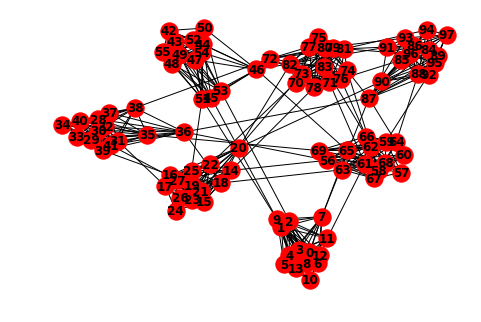
\includegraphics[scale=0.6]{static/graph_q7_n100_pin08_pout0011.png}
\caption{Graphe généré à partir des paramètres: $q=7$ $n=100$, $p_{in}=0.8$, $p_{out}=0.01$}
\end{figure}
\begin{figure}[H]
\centering
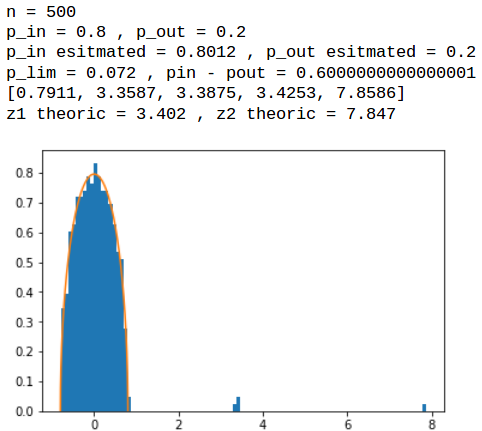
\includegraphics[scale=0.6]{static/spectral_q4_n500_pin08_pout02}
\caption{$q=4$, $n=500$, $\Delta p=0.6$}
\label{n500delta-05}
\end{figure}
\subsection{Limites du modèle}
Le première limite de ce modèle est que l'on est cantonné à des communautés de même taille $n_q$.
En effet si on change ce paramètre pour chacune des communautés alors le \autoref{th:1} n'est plus applicable, la somme des éléments de chaque vecteurs ligne du profile de variance n'est plus constant.\\

La deuxième contrainte est le fait que l'on doit toujours garder deux paramètres $p_{in}$ et $p_{out}$ indépendamment du nombre de communautés $n_q$ et du nombre de nœuds dans le graphe $n$.
Idéalement nous souhaiterions avoir un paramètre $p_{ij}$ correspondant à la probabilité d'avoir une arrête entre le nœud $i$ et le nœud $j$ et ce $\forall i<j$.\\
Une manière d'encoder ces paramètres est d'utiliser la relation suivante $p_{ij} = q_iq_jC_{\alpha}$
\begin{align}
	p_{ij} &= q_iq_jC_{g_ig_j}
\end{align}
Où $q_i$ est la probabilité intrinsèque du nœud $i$ à avoir une arrête, $g_i$ est la communauté correspondant au nœud $i$ et $C_{g_ig_j}$ est le facteur de correction par communauté.\\
Cette formalisation plus générale est très répandu dans la théorie de la détection de communauté spectrale.